%форматирование размера документа
\documentclass[11pt, a4paper]{article}

\usepackage{geometry}
% total - determines printable width, height
\geometry{ 
	a4paper, total={160mm,267mm}
}

%----text,fonts------------------------------------------------------------------------------------
\usepackage{mmap}
\usepackage[T2A]{fontenc}
\usepackage[utf8]{inputenc}
\usepackage[english, russian]{babel}
\usepackage{setspace}
\setstretch{0,9}

%----math,graphics---------------------------------------------------------------------------------
\usepackage{amsmath,amsfonts,amssymb}
\usepackage{amsthm}
\usepackage{listings}

\usepackage{tikz}
\usetikzlibrary{calc}
\usepackage{pgfplots}
\pgfplotsset{
	compat=1.17
}

\usepackage{graphicx}
\graphicspath{{image/}}

\usepackage{wrapfig}
\usepackage{tabularx}

% relative importing
\usepackage{import}

% module
\newcommand{\abs}[1]{\left\lvert#1\right\rvert}

\begin{document}

\import{}{titular.tex}
\newpage

\section{Описание метода. Расчетные формулы}

Метод Симпсона -- частный случай формул Ньютона-Котеса при $k = 2$. То есть пусть требуется найти 
вычислить интеграл 
\[
y = \int_a^b f(x)
\]

выбрав шаг 
\[
  h = \dfrac{b - a}{n}
\]
Тогда разобьем отрезок с помощью равноотстоящих точек $x_i = a + h * i$ на n равных частей.

Заменяя функцию $y_i = f(x_i)$ интерполяционным полиномом Лагранжа, который позволяет через 
заданное количество точек провести кривую получим приближенную квадратурную формулу.
\[
  \int_{x_0}^{x_n} y dx = \sum_{i = 0}^{n} A_i y_i
\]

Теперь если в эту формулу добавить постоянные коэффициенты Котеса, об этом рассказано в Демидовиче, то получим 
формулу
\[
  \int_{a}^b y dx = (b-a) * \sum_{i = 0}^n H_i y_i
\], 
где $H_i$ - коэффициент Котеса.

А теперь, если в этой формуле принять $n = 2$, то получим формулу Симпсона для нахождения 
значения интеграла функции. Коротко, мы разделяем отрезок $[a, b]$ на $n$ частей и проводим
через них параболы. 

То есть формула для 3-х точек будет выглядеть следующим образом  
\[
  \int_{x_0}^{x^n} y dx = \dfrac{h}{3} * (y_0 + 4 * y_1 + y_2)
\]
\medskip

Теперь рассмотрим общий случай. Пусть $n = 2*m$ четное число и $f(x_i)$ $(i = 0, 1, 2, \ldots, n)$ - значения функций в точках.
Сами точки являются равноотстоящими и определяются по формуле, указанной выше. Тогда применяя 
формулу к удвоенному промежутку $[x_0 x_2], [x_2 x_4] \\ \ldots [x_{n-2} x_n]$ будем иметь.

\begin{equation*}
  \int_a^b y dx = \dfrac{h}{3} (y_0 + 4y_1 + y_2) + \dfrac{h}{3} (y_2 + 4y_3 + y_4) + \ldots
  + \dfrac{h}{3} (y_{n-2} + 4y_{n-1} + y_n) 
\end{equation*}

Введя обозначения 
\begin{align*}
  \sigma_1 &= y_1 + y_3 + \ldots + y_{n-1} \\
  \sigma_2 &= y_2 + y_4 + \ldots + y_n
\end{align*}

запишем формулу в укороченном виде:

\begin{equation*}
  \int_a^b y dx = \dfrac{h}{3} [(y_0 + y_n) + 4 \sigma_1 + 2 \sigma_2)]
\end{equation*}


\section{Блок схема численного метода.}

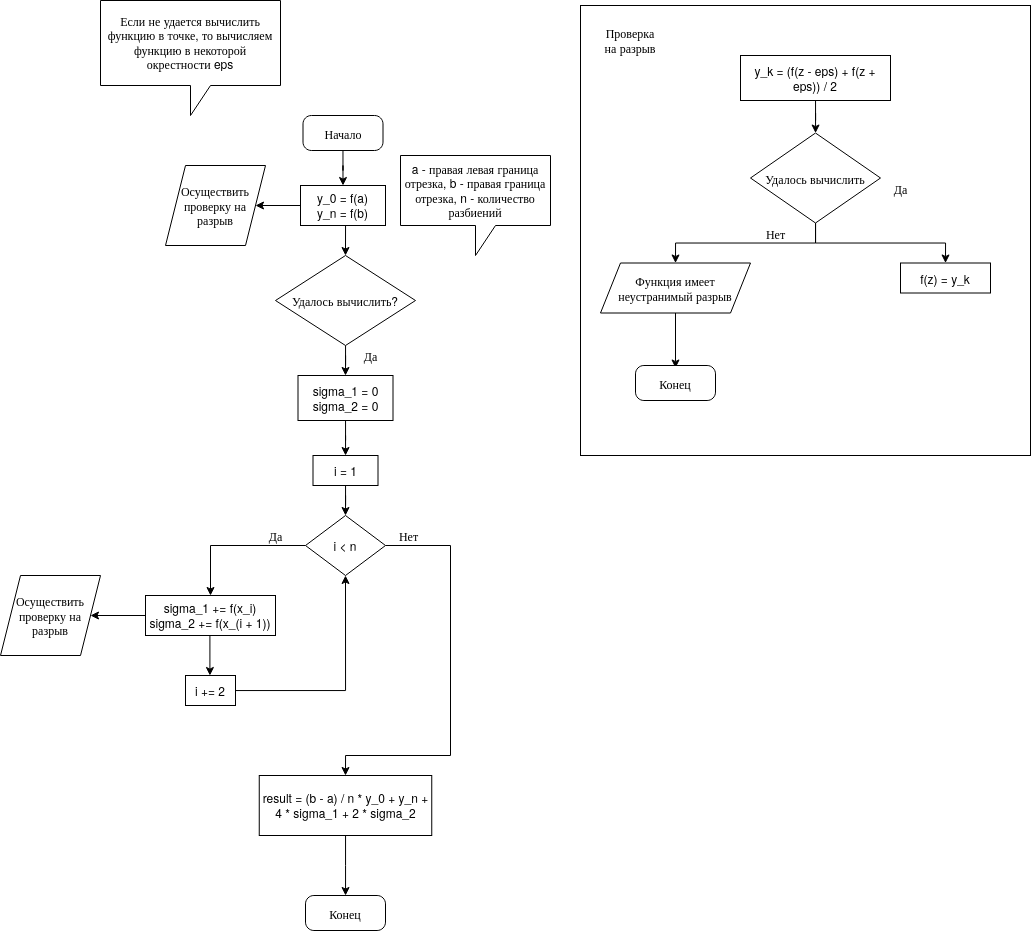
\includegraphics[width=\linewidth]{draw.png}

\bigskip
\section{Листинг реализованного численного метода.}

\begin{verbatim}
def _calculate_integral(equation: Node, range_min, range_max, step, var_lst):
    y0 = calculate(equation, {var_lst[0]: range_min})
    yn = calculate(equation, {var_lst[0]: range_max})
    n = int((range_max - range_min) / step)

    sigma1 = sum( [calculate(
      equation, {var_lst[0]: range_min + step * i}) for i in range(1, n, 2)])
    sigma2 = sum([calculate(
      equation, {var_lst[0]: range_min + step * i}) for i in range(2, n, 2)])

    return (step / 3) * (y0 + yn + 4 * sigma1 + 2 * sigma2)
\end{verbatim}

\newpage
\section{Примеры и результаты работы программы на разных данных.}

\noindentВвод данный через ifile-ofile:
\begin{verbatim}
data/task-3/input.json
[
  {
  "equation": [
    "x^2 + 5",
    "x^3"
  ],
  "data": {
    "range_min": -5,
    "range_max": 10,
    "step": 0.001
    }
  }
]

data/task-3/output.json
[
    {
        "result": 449.99999999999915,
        "r1": 1.6653345369377348e-15,
        "r2": 0.0,
        "r": 1.6653345369377348e-15
    },
    {
        "result": 2343.749999999999,
        "r1": 1.6653345369377348e-15,
        "r2": 0.0,
        "r": 1.6653345369377348e-15
    }
]
\end{verbatim}

\bigskip
\noindentВвод данных через stdin-stdout:
\begin{verbatim}
/usr/bin/python3.9 

Enter the equation [1]: x^2 + 10 * x + 5
Enter the left border: -12
Enter the right border: 12
Enter step: 0.001
Finish input? Y/N: y
Equation #1:
        Integral:       1272.00000000:
        Error R1:       2.66453526e-15:
        Error R2:       0.00000000e+00:
        Error R:        2.66453526e-15:

\end{verbatim}

\section{Вывод.}

В ходе выполнения данной лабораторной работы я познакомился с тем, каким образом можно 
считать значения интеграла от функции с помощью метода Симпсона. Кроме того, для того, чтобы
должным образом понимать, откуда была взята данная формула, разобрался с квадратурными формулами
Ньютона-Котеса (метод Симпсона есть частный случай при $n=3$, метод трапеций при $n = 2$), а также
с соответствующим интерполяционным полиномом Лагранжа.

\medskip
Для вычисления значения функции в точках устанимого разрыва следовал следующему алгоритму: 
вычислял значение функции в некоторой окрестности радиуса $\epsilon$ и находил среднее значение, определял $(f(x + \epsilon) 
+ f(x - \epsilon)) / 2$. 

\medskip
Кроме того, для более корректного определения значений измерений, расчитывал пределельную погрешность.
Для метода Симпсона с сравнении с методом трапеций и методом прямоугольников она имеет меньший порядок,
поскольку при нахождении площади некоторого сектора ширины $h$ функция, ограничивающая сверху данную
область, имеет вид параболы, в то время как для других предствленных методом она имеет форму прямой 
линии, соответственно, точность измерений будет больше.

\smallskip
Приводя конкретные значения предельных абсолютных погрешностей:

\smallskip
\textbullet~Метод средних прямоугольников: $\abs{R_1} \le \max_{x \in [a, b]}\abs{f''(x)} \dfrac{(b-a)^3}{24 n^2}$

\smallskip
\textbullet~Метод трапеций: $\abs{R_1} \le \max_{x \in [a, b]}\abs{f''(x)} \dfrac{(b-a)^3}{12 n^2}$

\smallskip
\textbullet~Метод Симпсона: $\abs{R_1} \le \max_{x \in [a, b]}\abs{f''''(x)} \dfrac{(b-a)^5}{180 n^4}$

\medskip
Также не следует забывать про набегающую погрешность, возникающую из-за ограниченности разрядной
сетки компьютера. Так для метода Симпсона данная величина равняется
\begin{equation*}
  \abs{R_2} \le (b - a) * \epsilon
\end{equation*}, где $\epsilon$ - величина, обозначающая погрешность вычислений для каждой итерации нахождения значения функции. Так для 64-разрядной
машины $\epsilon \le 1/2^{52}$.

\medskip
Таким образом, предельная абсолютная погрешность измерений: $\abs{R} \le \abs{R_1} + \abs{R_2}$.
\end{document}
